\begin{textarea}[]
\only<1>{
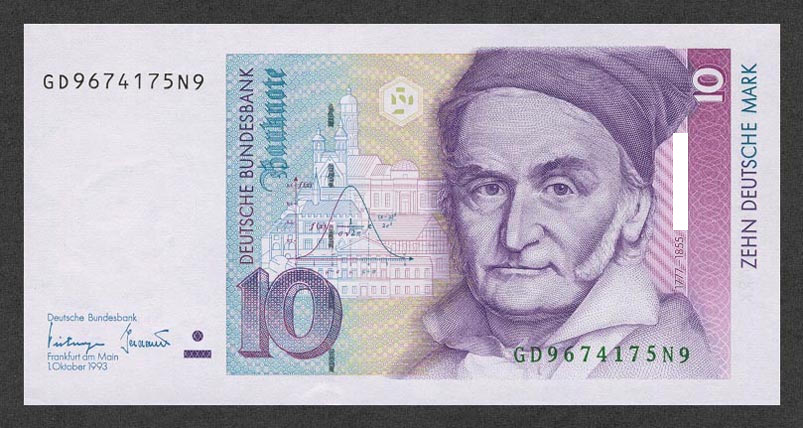
\includegraphics[height=0.5\linewidth]{categories/media/10_DM_Serie4_Vorderseite}
}
\only<2>{
Who is Carl Friedrich Gau{\ss}?
}
\end{textarea}

\begin{textarea}[]
\only<1>{
\begin{columns}[c] 
    \column{.5\textwidth} 
     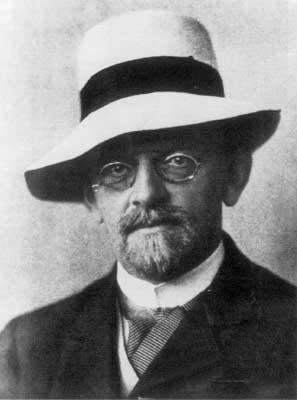
\includegraphics[height=0.5\linewidth]{categories/media/Hilbert}
    \column{.5\textwidth}
     This German mathematician is said to be one of the most influential ones, even though he left us with $23$ unsolved problems.
    \end{columns}
}
\only<2>{
Who is David Hilbert?
}
\end{textarea}

\begin{textarea}[]
\only<1>{
\begin{columns}[c] 
    \column{.5\textwidth} 
     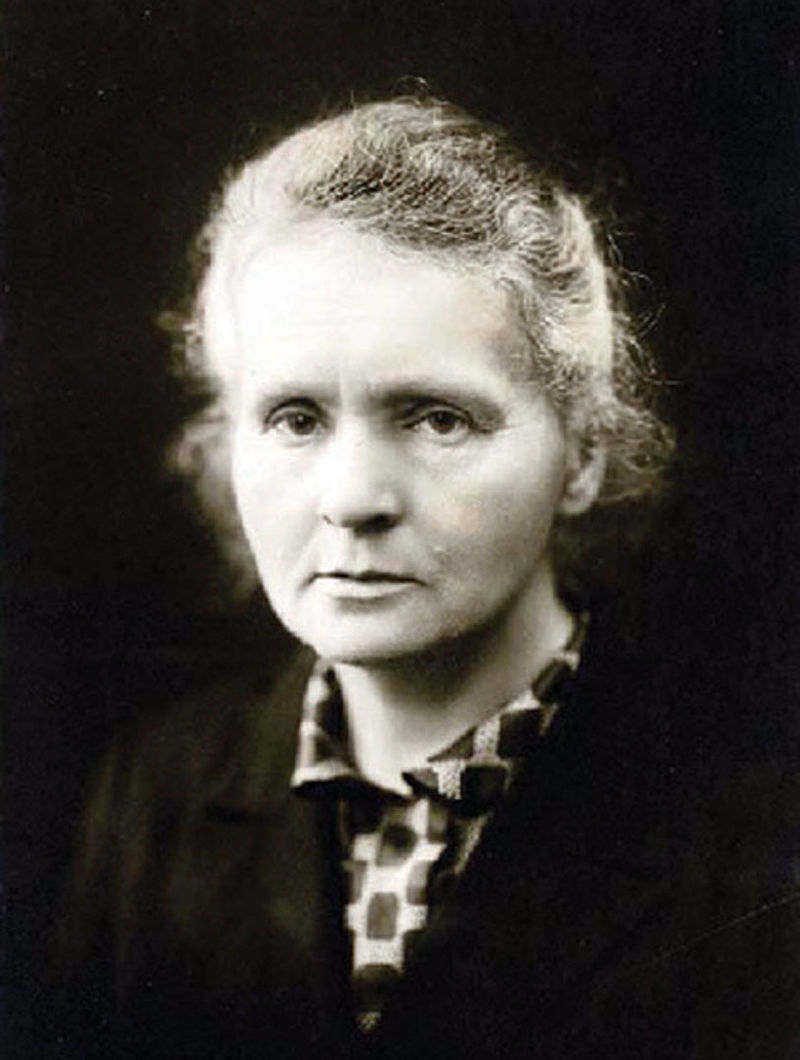
\includegraphics[height=1.0\linewidth]{categories/media/MarieCurie}
    \column{.5\textwidth}
     This Polish scientist was the first to be rewarded with a Nobel prize.
    \end{columns}
}
\only<2>{
Who is Marie Curie?
}
\end{textarea}

\begin{textarea}[]
\only<1>{
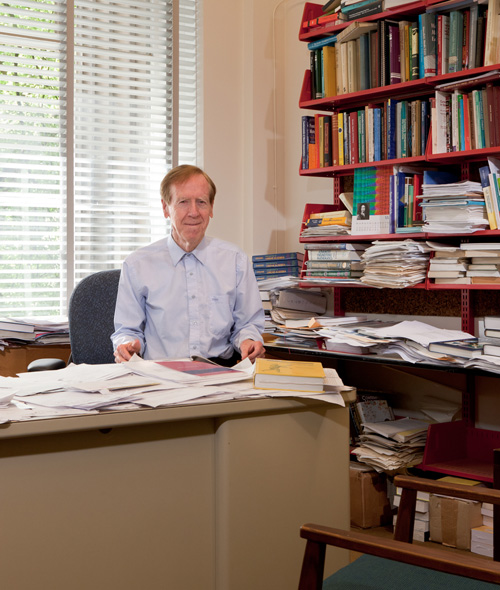
\includegraphics[height=0.5\linewidth]{categories/media/Strang8}
}
\only<2>{
Who is Gilbert Strang?
}
\end{textarea}

\begin{textarea}[]
\only<1>{
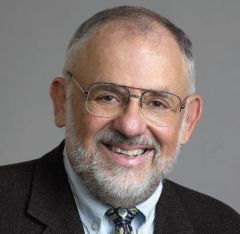
\includegraphics[height=0.5\linewidth]{categories/media/CleveMoler}
}
\only<2>{
Who is Cleve Moler?
}
\end{textarea}

\begin{textarea}[]
\only<1>{
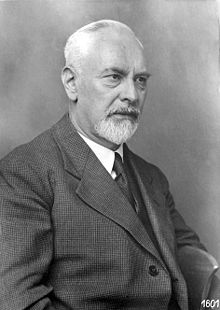
\includegraphics[height=0.5\linewidth]{categories/media/LudwigPrandtl}
}
\only<2>{
Who is Ludwig Prandtl?
}
\end{textarea}